\section{Quantitative Evaluation}\label{sec:eval}
We first test the common-model operating regimes and descriptive similarity to native methods (RQ1), then continuous budget feasibility and inverse queries (RQ2). Retained shared-input comparisons and source-linked cases examine practical consequences (RQ3). New common-QP measurements, frontier witnesses and earlier P/R measurements retain separate result identities and guarantees.

\subsection{Data Sets, Protocol, and Measures}
Table~\ref{tab:datasets_main} lists all nine evaluated inputs, their scalar fields, spatial dimensions, grids, sample counts, extracted leaves, and tree types. The five planar temporal sequences contain 614 frames: Storms (118 half-day pressure fields), Wildfires (30 two-day fire-radiative-power aggregates), OLR (60 daily fields), PM2.5 (366 fields covering all of 2000), and synthetic Ring (40 frames)~\cite{Hersbach:2020:ERA5,Franke:2021:1DP,NOAA:OLR,Dong:2026:PM25,Koepp:2023:TMTM}. The separate 744-hour Storms overview and 64-frame mirror control do not enter the 614-frame small-tree statistics.

The remaining planar inputs are the original author $64\times64$ static Nucleon slice and 21 static sections of an explicitly reconstructed Benzene point-charge potential~\cite{Koepp:2023:TMTM,Jorgensen:2013:BOSS,Inviwo:BenzeneGeometry}. Tangaroa subsequently supplies 201 original-grid three-dimensional velocity-magnitude fields, and Cylinder supplies 102 three-dimensional $Q$ fields derived from public velocity volumes~\cite{Popinet:2004:Tangaroa,Camarri:2005:Cylinder,Weinkauf:SquareCylinder}. Section index is not physical time. All nine inputs appear together in Table~\ref{tab:tradeoff}; input dimensions and independent populations remain explicit. The seven temporal inputs comprise 917 fields, without forming a pooled accuracy score.

All methods share each input's processed fields, extrema, supports, and overlap matches. Retained temporal-construction comparisons use shared-input TMTM and ST-MTM reimplementations, RG-MTM-P, and RG-MTM-R at $\kappa/\Delta_F=0.20$. ST-MTM uses uniform distance weights, $r=0.95$, and temporal weight $0.5$ (Ring: $1.5$). The previously omitted Nucleon, Benzene, Tangaroa and Cylinder comparisons have now been computed on all 325 retained inputs with these fixed generic settings and 32768-row profiles. Nucleon uses base mode; Benzene propagates across spatial sections without assigning physical time. For the volumetric extension, the same equations use three-dimensional centroid distances. A deterministic equal-level binary refinement handles multifurcations while preserving all source leaf supports and labelled merge levels; it restricts the admissible leaf orders and is an implementation assumption. Supplement S3 records the equations, width units, solver checks and complete results; this is a shared-input extension rather than reproduction of unpublished original presets. The RG modes share geometry and secondary objectives. An independent 148-frame Storms/Wildfires audit matches 486 TMTM branch decisions and 1118 interval/anchor records to the official C++ core, and checks ST-MTM objectives, constraints, and rendered topology (Supplement S7). Supplemental controls comprise native Hilbert/Morton traversals, packed reference sorting, fixed axes, and exact reference projection. Supplements S2, S6, and S9 retain all acquisition, smoothing, cropping, boundary, simplification, and solver settings.

\begin{table*}[t]
\caption{All nine inputs evaluated with the shared error definitions. Source dimension describes the input, not the two-dimensional map output.}\label{tab:datasets_main}
\centering\footnotesize\setlength{\tabcolsep}{4pt}
\begin{tabular}{lllrlll}\toprule
Data & Input & Scalar field & Processed grid & Samples & Leaves & Tree\\\midrule
Storms & 2-D & Mean sea-level pressure & $49\times49$ & 118 frames & 1--8 & Join\\
Wildfires & 2-D & $\log(1+\mathrm{FRP})$ & $64\times64$ & 30 frames & 6--11 & Split\\
OLR & 2-D & Outgoing longwave radiation & $49\times49$ & 60 frames & 2--8 & Join\\
PM$_{2.5}$ & 2-D & PM$_{2.5}$ concentration & $49\times49$ & 366 frames & 1--7 & Split\\
Ring & 2-D & Synthetic ring intensity & $14\times14$ & 40 frames & 1--7 & Split\\
Tangaroa & 3-D & Velocity magnitude & $300\times180\times120$ & 201 frames & 18--93 & Join\\
Cylinder & 3-D & Q criterion & $135\times64\times48$ & 102 frames & 4--75 & Split\\
Nucleon & 2-D & Nucleon scalar & $64\times64$ & 1 slice & 13 & Split\\
Benzene & 2-D & Reconstructed electrostatic potential & $61\times61$ & 21 sections & 5--10 & Join\\
\bottomrule\end{tabular}
\par\smallskip{\footnotesize\raggedright Storms, Wildfires, OLR and PM$_{2.5}$ are observed fields; Ring is synthetic. Tangaroa and Cylinder are volumetric simulations. Cylinder Q is computed on the original $192\times64\times48$ velocity grid before the $135\times64\times48$ crop. Nucleon is one author-provided static planar slice; Benzene is a reconstructed point-charge potential evaluated on 21 static sections. Seven temporal sequences contain 917 frames; static sections and the independent mirror control are separate populations.\par}
\end{table*}


\paragraph{Reference order and actual displacement.}
Normalized Reference-Order Error (NROE) evaluates the displayed anchor order $\pi_t$ independently of native scales and widths:
\begin{equation}
\begin{aligned}
 \mathrm{NROE}_t&=\frac{\max\{0,\max_{r<s}(q_{\pi_r}^t-q_{\pi_s}^t)\}}{2L},\\
 \mathrm{NROE}&=\operatorname{mean}_t\mathrm{NROE}_t .
\end{aligned}\label{eq:order_metric}
\end{equation}
It is the smallest maximum displacement after monotone calibration, with stable tie-breaking for coincident anchors; single-leaf frames have zero order error. Actual RG coordinates use $E_{\rm pool}=\sum_{t,i}|u_i^t-q_i^t|/(L\sum_t n_t)$ and $E_\infty=\max_{t,i}|u_i^t-q_i^t|/L$, computed from continuous layouts. These separate order compatibility from achieved position. The same continuous definitions apply to all nine inputs, including the volumetric and static cases; they do not substitute the older rendered, frame-averaged MAE.

\paragraph{Merge levels.}
Normalized Merge-Level Error is $D_t=d_{\rm top}(\psi_t,T_t)/\Delta_F$, using a fixed processed scalar range for the sequence. NMLE$_{\rm mean}$ averages framewise worst-pair errors; NMLE$_{\rm max}$ gives the worst frame. Values in Table~\ref{tab:tradeoff} are measured from filled-raster barriers. The analytical $\delta^*$ supplies the corresponding fixed-order prediction. This metric evaluates merge thresholds for corresponding leaves; it does not measure all changes to the scalar distribution or thresholded spatial regions.

\paragraph{Motion and geometry.}
A tracked pair supplies a clear approach/separation event when its two- or three-dimensional source-space Euclidean distance changes by more than 2\% of domain diagonal across two steps. The displayed decision uses anchor-distance change and a 2\% threshold of the method's sequence-wide occupied range, except Cylinder, whose retained protocol uses 2\% of the fixed full canvas for every method. This threshold convention is also used for its new ST-MTM run. Motion error ME counts reversals plus misses among shared $N_{\rm clear}$ events. Four-step circular temporal blocks give paired bootstrap intervals. Support-centroid scale-normalized stress (SNS), trustworthiness (TW), and full-canvas temporal displacement (TD) quantify additional geometric properties; their definitions and complete results are in Supplement S3. Motion counts are geometric diagnostics of overlap-linked extrema. Small event populations and static inputs are reported explicitly, and no aggregate accuracy is inferred from averaging datasets with different event counts.

\begin{table*}[t]
\caption{Complete shared-input evaluation, grouped by method. All 2-D inputs precede the 3-D volumes in every panel.}\label{tab:tradeoff}
\centering\footnotesize\setlength{\tabcolsep}{2pt}
\textit{(a) Reference order, motion and merge-level cost}\par\smallskip
\begin{tabular*}{\textwidth}{@{\extracolsep{\fill}}lrrrrrrrrrrr@{}}\noalign{\hrule height .8pt width \textwidth\vskip 2.5pt}
 & & \multicolumn{2}{c}{TMTM} & \multicolumn{2}{c}{ST-MTM} & \multicolumn{2}{c}{RG-MTM-P (ours)} & \multicolumn{4}{c}{RG-MTM-R (ours)}\\
\cmidrule(lr){3-4}\cmidrule(lr){5-6}\cmidrule(lr){7-8}\cmidrule(lr){9-12}
Data & $N_{\rm clear}$ & NROE$\downarrow$ & ME$\downarrow$ & NROE$\downarrow$ & ME$\downarrow$ & NROE$\downarrow$ & ME$\downarrow$ & NROE$\downarrow$ & ME$\downarrow$ & NMLE$_{\rm mean}\downarrow$ & NMLE$_{\rm max}\downarrow$\\\midrule
Storms & 104 & 19.23 & 0.471 & 16.28 & 0.413 & 3.77 & 0.231 & 1.16 & 0.183 & 1.47 & 26.07\\
Wildfires & 112 & 29.30 & 0.393 & 24.02 & 0.357 & 5.83 & 0.321 & 0.34 & 0.312 & 3.96 & 19.56\\
OLR & 56 & 19.31 & 0.446 & 17.21 & 0.214 & 0.89 & 0.054 & 0.00 & 0.054 & 1.10 & 33.56\\
PM2.5 & 95 & 12.87 & 0.453 & 11.60 & 0.516 & 0.98 & 0.442 & 0.01 & 0.495 & 0.18 & 4.67\\
Ring & 124 & 7.18 & 0.645 & 10.39 & 0.347 & 2.66 & 0.315 & 0.13 & 0.129 & 2.73 & 12.35\\
Nucleon & -- & 11.9048 & -- & 11.9048 & -- & 2.3810 & -- & 2.3810 & -- & 0.0000 & 0.0000\\
Benzene & -- & 50.0000 & -- & 50.0000 & -- & 4.2063 & -- & 0.0000 & -- & 0.0025 & 0.0080\\
Tangaroa & 6755 & 20.09 & 0.975 & 21.34 & 0.700 & 9.61 & 0.547 & 0.02 & 0.305 & 14.44 & 31.02\\
Cylinder & 3196 & 26.62 & 0.670 & 17.77 & 0.460 & 12.26 & 0.373 & 0.08 & 0.189 & 2.81 & 14.28\\
\bottomrule\end{tabular*}
\par\medskip
\textit{(b) Standard geometry and temporal stability}\par\smallskip
\begin{tabular*}{\textwidth}{@{\extracolsep{\fill}}lrrrrrrrrrrrr@{}}\noalign{\hrule height .8pt width \textwidth\vskip 2.5pt}
 & \multicolumn{3}{c}{TMTM} & \multicolumn{3}{c}{ST-MTM} & \multicolumn{3}{c}{RG-MTM-P (ours)} & \multicolumn{3}{c}{RG-MTM-R (ours)}\\
\cmidrule(lr){2-4}\cmidrule(lr){5-7}\cmidrule(lr){8-10}\cmidrule(lr){11-13}
Data & SNS$\downarrow$ & TW$_1\uparrow$ & TD$\downarrow$ & SNS$\downarrow$ & TW$_1\uparrow$ & TD$\downarrow$ & SNS$\downarrow$ & TW$_1\uparrow$ & TD$\downarrow$ & SNS$\downarrow$ & TW$_1\uparrow$ & TD$\downarrow$\\\midrule
Storms & 0.0799 & 0.8243 & 10.1108 & 0.0297 & 0.9653 & 7.1607 & 0.1186 & 0.7771 & 27.3609 & 0.1097 & 0.7554 & 23.8891\\
Wildfires & 0.2210 & 0.8170 & 11.2034 & 0.0786 & 0.9195 & 7.9585 & 0.0831 & 0.8793 & 8.0342 & 0.0579 & 0.8725 & 3.2487\\
OLR & 0.1419 & 0.8135 & 8.7479 & 0.0062 & 0.9751 & 2.3304 & 0.0121 & 0.9587 & 8.9011 & 0.0093 & 0.9634 & 8.5023\\
PM2.5 & 0.0509 & 0.7596 & 38.7546 & 0.0256 & 0.9223 & 7.7763 & 0.0640 & 0.7492 & 76.3170 & 0.0524 & 0.7291 & 68.7114\\
Ring & 0.1706 & 0.7067 & 1.3436 & 0.0803 & 0.9172 & 2.3641 & 0.1637 & 0.7087 & 3.5977 & 0.1423 & 0.7149 & 2.3512\\
Nucleon & 0.3122 & 0.9161 & -- & 0.0506 & 0.9860 & -- & 0.1325 & 0.8951 & -- & 0.1325 & 0.8951 & --\\
Benzene & 0.1750 & 0.6264 & -- & 0.1284 & 0.6254 & -- & 0.1588 & 0.4972 & -- & 0.1570 & 0.5258 & --\\
Tangaroa & 0.5255 & 0.6701 & 64.8553 & 0.1655 & 0.8137 & 138.5519 & 0.3571 & 0.7271 & 158.2670 & 0.3353 & 0.7458 & 39.7093\\
Cylinder & 0.2956 & 0.8017 & 85.0339 & 0.1346 & 0.8989 & 43.1663 & 0.1393 & 0.7838 & 72.3427 & 0.0399 & 0.8912 & 29.1130\\
\bottomrule\end{tabular*}
\par\medskip
\textit{(c) Continuous reference displacement and static-section coherence}\par\smallskip
\begin{tabular*}{\textwidth}{@{\extracolsep{\fill}}lrrrrrrrr@{}}\noalign{\hrule height .8pt width \textwidth\vskip 2.5pt}
 & TMTM & ST-MTM & \multicolumn{3}{c}{RG-MTM-P (ours)} & \multicolumn{3}{c}{RG-MTM-R (ours)}\\
\cmidrule(lr){2-2}\cmidrule(lr){3-3}\cmidrule(lr){4-6}\cmidrule(lr){7-9}
Data & SD$\downarrow$ & SD$\downarrow$ & $E_{\rm pool}\downarrow$ & $E_\infty\downarrow$ & SD$\downarrow$ & $E_{\rm pool}\downarrow$ & $E_\infty\downarrow$ & SD$\downarrow$\\\midrule
Storms & -- & -- & 4.13 & 26.19 & -- & 2.14 & 18.46 & --\\
Wildfires & -- & -- & 3.18 & 20.48 & -- & 0.80 & 6.64 & --\\
OLR & -- & -- & 1.00 & 17.14 & -- & 0.57 & 1.69 & --\\
PM2.5 & -- & -- & 1.87 & 20.26 & -- & 0.76 & 5.86 & --\\
Ring & -- & -- & 2.43 & 11.90 & -- & 0.71 & 2.52 & --\\
Nucleon & -- & -- & 1.92 & 3.43 & -- & 1.92 & 3.43 & --\\
Benzene & 4.1118 & 1.9658 & 1.60 & 15.39 & 2.4060 & 0.52 & 1.75 & 0.9601\\
Tangaroa & -- & -- & 5.01 & 16.86 & -- & 1.18 & 8.02 & --\\
Cylinder & -- & -- & 5.40 & 32.08 & -- & 0.55 & 5.27 & --\\
\bottomrule\end{tabular*}
\par\smallskip{\footnotesize\raggedright NROE and continuous $E$ are percentages of reference extent; NMLE is a percentage of the fixed processed scalar range. ME is the error fraction over the shared $N_{\rm clear}$ events (lag 2; 2\% source-distance threshold). Cylinder retains its 2\%-of-full-canvas display threshold; other temporal inputs use the method-specific occupied range. SNS uses scale-fitted squared centroid-distance residuals; TW uses $k=1$ on valid frames. TD sums matched displacements in full-canvas units. SD is the separately named adjacent-section displacement, available only for Benzene (170 spatial matches). -- denotes an inapplicable metric; native axes have no direct-reference $E$ without calibration. TMTM, ST-MTM and P have zero measured NMLE. R uses $\kappa=0.2\Delta_F$, an eligibility threshold rather than an achieved-error cap. Protocols and eligible counts are in Supplement S3.\par}
\end{table*}


\subsection{Established Geometry and Stability Metrics on 2-D Inputs}
We additionally evaluate the criteria used by ST-MTM~\cite{STMTM:2026}: scale-normalized stress (SNS), trustworthiness (TW), and temporal displacement (TD). SNS minimizes squared centroid-distance residuals over one positive scale per frame, without a square root; lower is better. TW penalizes introduced neighbours by their original-space rank; higher is better. We fix $k=1$ across all inputs and average only frames satisfying $k<n/2$. TD is the sum of matched-anchor absolute changes after one fixed full-canvas mapping per sequence, not a frame average or occupied-range normalization. Supplement S3 lists all eligible frame counts and exact formulas.

The completed planar comparison distinguishes alignment from relative geometry. ST-MTM retains better SNS, TW and TD than R20 on Storms, OLR and annual PM2.5. R20 has lower SNS on Wildfires and lower TD on Wildfires and Ring, while its TW remains lower on all five temporal inputs. These complementary outcomes support a controlled reference--geometry trade-off, rather than universal superiority.

Both static planar inputs now have all four methods' SNS and TW. Nucleon ST-MTM attains SNS 0.0506 and TW 0.9860; P/R attain 0.1325 and 0.8951 despite their lower reference-order error. On Benzene, ST-MTM SNS is 0.1284 versus R20's 0.1570, whereas R20 has smaller summed adjacent-section displacement (0.9601 versus 1.9657 canvas widths over the same 170 matches). Temporal ME and TD are undefined for both static inputs. Section displacement is a separate spatial-coherence measurement, not a zero temporal error.

\subsection{Operating Regimes of One Model (RQ1)}
We recompute topology--time, topology--geometry, and reference-guided layouts at topology allowances 0, 2\% and 10\% on the same five planar sequences. This produces 3070 layouts from 614 frames. All five settings share each frame's candidate pool, widths, canvas, scalar range, source-value renderer and convex QP implementation. They differ only in the controls in Table~\ref{tab:profiles}; the main regime comparison disables the reference cap ($B=\infty$). A separate Ring grid fixes the reference objective and evaluates all nine combinations of $\varepsilon\in\{0,0.02,0.1\}$ and $B\in\{\infty,0.1,0.05\}$.

The common-model search covers all permutations on 496 frames; the other 118 frames use recorded candidate pools. Across the five settings it evaluates 15141 admissible fixed-order QPs. These coverage counts describe the new QP experiment, not the independently exhaustive frontier experiment below. Selected continuous layouts satisfy their topology and position caps, and the largest normalized candidate-objective gap bound is 1.2e-06. Independent saved-witness checks reconstruct the objective, constraints and selected-order first-order gaps.

Geometry activation reduces the geometry residual relative to the topology--time setting on all five tested inputs. Reference activation greatly reduces absolute reference error, while changing the temporal target from stationary alignment to projected-motion following. These changes express distinct priorities rather than a universal quality ranking. The 2\% and 10\% scalar allowances further reduce pooled reference error on all five sequences in this run, but no monotonic improvement in every component or recomputed temporal history is claimed. Table~\ref{tab:unified_regimes} reports all component measures; Figures~\ref{fig:unified_regimes}--\ref{fig:unified_budget_grid} show the resulting maps.

The shared-input native TMTM and ST-MTM reimplementations are run independently on Ring and Storms. Descriptive similarity uses labelled-pair order agreement and anchor RMSE after one sequence-wide affine gauge fit, including reflection. The fit does not modify the underlying layouts or any reference-error metric. Table~\ref{tab:unified_similarity} reports the results. The topology--time regime is an anchor-alignment surrogate for TMTM, and the topology--geometry regime uses common interval rules instead of ST-MTM's native allocation. In particular, low Storms agreement with native ST-MTM exposes a substantive difference; common design priorities do not imply universally close coordinates. Independent baseline audits retain their separate evidence role in Supplement S7.

The unit tests also isolate an important control: a zero reference weight can still leave a reference-dependent hard position cap. Explicitly disabling that cap recovers geometry-only behavior on a two-feature example, and the canonical null-space rule resolves free newborn coordinates without changing the primary objective. These checks support the interpretation of the parameter regimes rather than native-algorithm equivalence.

\begin{table*}[t]
\caption{New common-model results on all 614 planar frames, with five settings each (3070 layouts). All numbers are percentages: pooled absolute reference error (R-MAE), root mean framewise geometry/temporal squared residual (G-RMS, stationary S-RMS and projected-motion M-RMS), and worst continuous labelled merge error (Top-max). Geometry and temporal quantities use the common fixed canvas, not native-baseline scales. Empty pair/match terms contribute zero. First-frame temporal terms are zero. Different components express competing priorities; lower reference error need not improve every score.}\label{tab:unified_regimes}
\centering\small
\begin{tabular}{llrrrrr}\toprule
Input & Regime & R-MAE & G-RMS & S-RMS & M-RMS & Top-max\\\midrule
Ring & Topology--time & 27.37 & 18.15 & 0.28 & 2.64 & 0.00 \\
Ring & Topology--geometry & 29.75 & 5.88 & 2.66 & 3.67 & 0.00 \\
Ring & Reference, 0\% & 2.57 & 8.58 & 3.97 & 3.42 & 0.00 \\
Ring & Reference, 2\% & 2.28 & 8.41 & 3.33 & 2.66 & 1.49 \\
Ring & Reference, 10\% & 1.17 & 8.15 & 2.65 & 1.20 & 9.40 \\
Storms & Topology--time & 25.31 & 47.41 & 0.38 & 18.65 & 0.00 \\
Storms & Topology--geometry & 33.56 & 11.73 & 8.86 & 19.46 & 0.00 \\
Storms & Reference, 0\% & 6.09 & 20.68 & 20.67 & 9.50 & 0.00 \\
Storms & Reference, 2\% & 5.78 & 20.61 & 20.67 & 8.51 & 1.31 \\
Storms & Reference, 10\% & 5.06 & 19.91 & 20.04 & 6.82 & 8.51 \\
Wildfires & Topology--time & 16.67 & 29.88 & 1.02 & 2.83 & 0.00 \\
Wildfires & Topology--geometry & 13.94 & 8.62 & 7.05 & 7.07 & 0.00 \\
Wildfires & Reference, 0\% & 3.19 & 10.03 & 6.89 & 6.13 & 0.00 \\
Wildfires & Reference, 2\% & 2.72 & 9.65 & 6.26 & 5.29 & 1.85 \\
Wildfires & Reference, 10\% & 1.84 & 9.01 & 5.16 & 4.13 & 8.35 \\
OLR & Topology--time & 24.43 & 35.53 & 0.56 & 9.42 & 0.00 \\
OLR & Topology--geometry & 42.71 & 4.26 & 4.94 & 11.63 & 0.00 \\
OLR & Reference, 0\% & 1.31 & 4.93 & 9.14 & 2.45 & 0.00 \\
OLR & Reference, 2\% & 1.17 & 4.80 & 9.11 & 2.37 & 1.79 \\
OLR & Reference, 10\% & 1.04 & 4.52 & 9.06 & 2.28 & 5.15 \\
PM$_{2.5}$ & Topology--time & 21.71 & 21.60 & 0.74 & 21.88 & 0.00 \\
PM$_{2.5}$ & Topology--geometry & 25.03 & 6.40 & 4.38 & 22.24 & 0.00 \\
PM$_{2.5}$ & Reference, 0\% & 3.05 & 10.60 & 22.07 & 5.44 & 0.00 \\
PM$_{2.5}$ & Reference, 2\% & 2.43 & 9.93 & 21.98 & 4.40 & 1.81 \\
PM$_{2.5}$ & Reference, 10\% & 2.15 & 9.61 & 21.80 & 3.54 & 4.67 \\
\bottomrule\end{tabular}\end{table*}

\begin{table}[t]
\caption{Descriptive similarity of inspired regimes to their native comparison methods. One sequence-wide least-squares affine transform, including reflection, aligns native anchors to the inspired anchors; no framewise fit is used. Agreement counts non-tied labelled feature pairs. RMSE is a percentage of the common inspired canvas. Values measure similarity, not algorithm recovery.}\label{tab:unified_similarity}
\centering\small
\begin{tabular}{llrrr}\toprule
Input & Native & Order (\%) & RMSE (\%) & Pairs\\\midrule
Ring & TMTM & 80.6 & 1.37 & 346 \\
Ring & ST-MTM & 77.2 & 9.69 & 346 \\
Storms & TMTM & 72.5 & 5.98 & 596 \\
Storms & ST-MTM & 51.7 & 34.24 & 596 \\
\bottomrule\end{tabular}\end{table}


\subsection{True Error Budgets and Inverse Queries (RQ2)}\label{sec:budget_experiments}
We newly evaluate nine normalized topology allowances $\{0,0.005,0.01,0.02,0.05,0.1,0.2,0.5,1\}$ on the unchanged five-sequence input population of 614 frames. Every frame uses the same fixed reference, canvas and absolute width convention across the sweep. All permutations are evaluated up to $8!=40320$ orders: 603 frames are exhaustive. The remaining 11 Wildfires frames use the fixed candidate set in Section~\ref{sec:hard_budget}; their values are feasible upper bounds, not certified global minima. No frames are excluded from the reported means.

The run constructs 5526 LP-anchor/barrier witnesses and evaluates 3684 inverse queries at six position caps. Every returned continuous witness meets its declared scalar allowance. No frame's selected position cost increases as $\varepsilon$ increases. The inverse query reports failure when no admissible order meets the requested position cap; on a candidate-only frame this means that no witness was found, rather than global infeasibility. Exhaustive frames supply the stronger interpretation.
\begin{table*}[t]
\caption{New hard-budget experiments on all 614 planar temporal frames. Position columns report the temporal mean of the framewise minimax absolute position error, in percent of the fixed reference extent. These are not NROE or the achieved secondary-QP errors in the retained tables. Wildfires includes 11 candidate-only upper bounds. The inverse column counts frames with a witnessed solution at a 2\% position cap and unrestricted scalar allowance; it is not the count attainable at a 2\% topology cap.}\label{tab:budget_results}
\centering\small
\begin{tabular}{lrrrrr}\toprule
Input & Exact/total & $\varepsilon=0$ & $\varepsilon=2\%$ & $\varepsilon=10\%$ & $E_t(2\%)$ feasible\\\midrule
Storms & 118/118 & 4.326 & 3.499 & 1.889 & 115/118 \\
Wildfires & 19/30 & 6.178 & 3.482 & 1.926 & 30/30 \\
OLR & 60/60 & 0.960 & 0.639 & 0.332 & 60/60 \\
PM$_{2.5}$ & 366/366 & 1.282 & 0.533 & 0.121 & 358/366 \\
Ring & 40/40 & 2.876 & 1.688 & 0.112 & 40/40 \\
\bottomrule\end{tabular}
\end{table*}


At a genuine 2\% topology cap, mean minimax position error changes from 4.326\% to 3.499\% on Storms, 6.178\% to 3.482\% on Wildfires, 0.960\% to 0.639\% on OLR, 1.282\% to 0.533\% on annual PM2.5, and 2.876\% to 1.688\% on Ring. These quantities are continuous per-frame minimax values, not NROE and not the achieved coordinates of the retained secondary-QP layouts. Figure~\ref{fig:budget_response} shows the budget response and illustrative Ring maps generated from the saved witnesses.

At a requested position cap of 2\% with unrestricted scalar allowance, the system finds witnesses in 115/118 Storms, 30/30 Wildfires, 60/60 OLR, 358/366 PM2.5 and 40/40 Ring frames. The three unsuccessful Storms and eight PM2.5 frames were exhaustively searched: their fixed widths and canvas prevent the target even after releasing topology. The inverse query returns a different minimum topology allowance for each feasible frame; these counts do not imply that a 2\% topology cap suffices. A sequence-wide feasibility claim uses the worst frame, whereas Table~\ref{tab:budget_results} reports temporal means.

\paragraph{Scope and controls.}
These experiments establish the continuous non-strict framewise budget behavior. They do not reuse the earlier motion scores as measurements of the new LP witnesses, establish a temporal-QP optimum, or certify a rounded raster under the same cap. The Ring illustrations have finite display resolution and are not used for the numerical guarantees. Existing P/R results below remain separate temporal-construction operating points; their parameter $\kappa$ is an eligibility threshold rather than $\varepsilon$.


\subsection{Retained Position Certificates and Scalar Correction}
\begin{figure*}[t]
\centering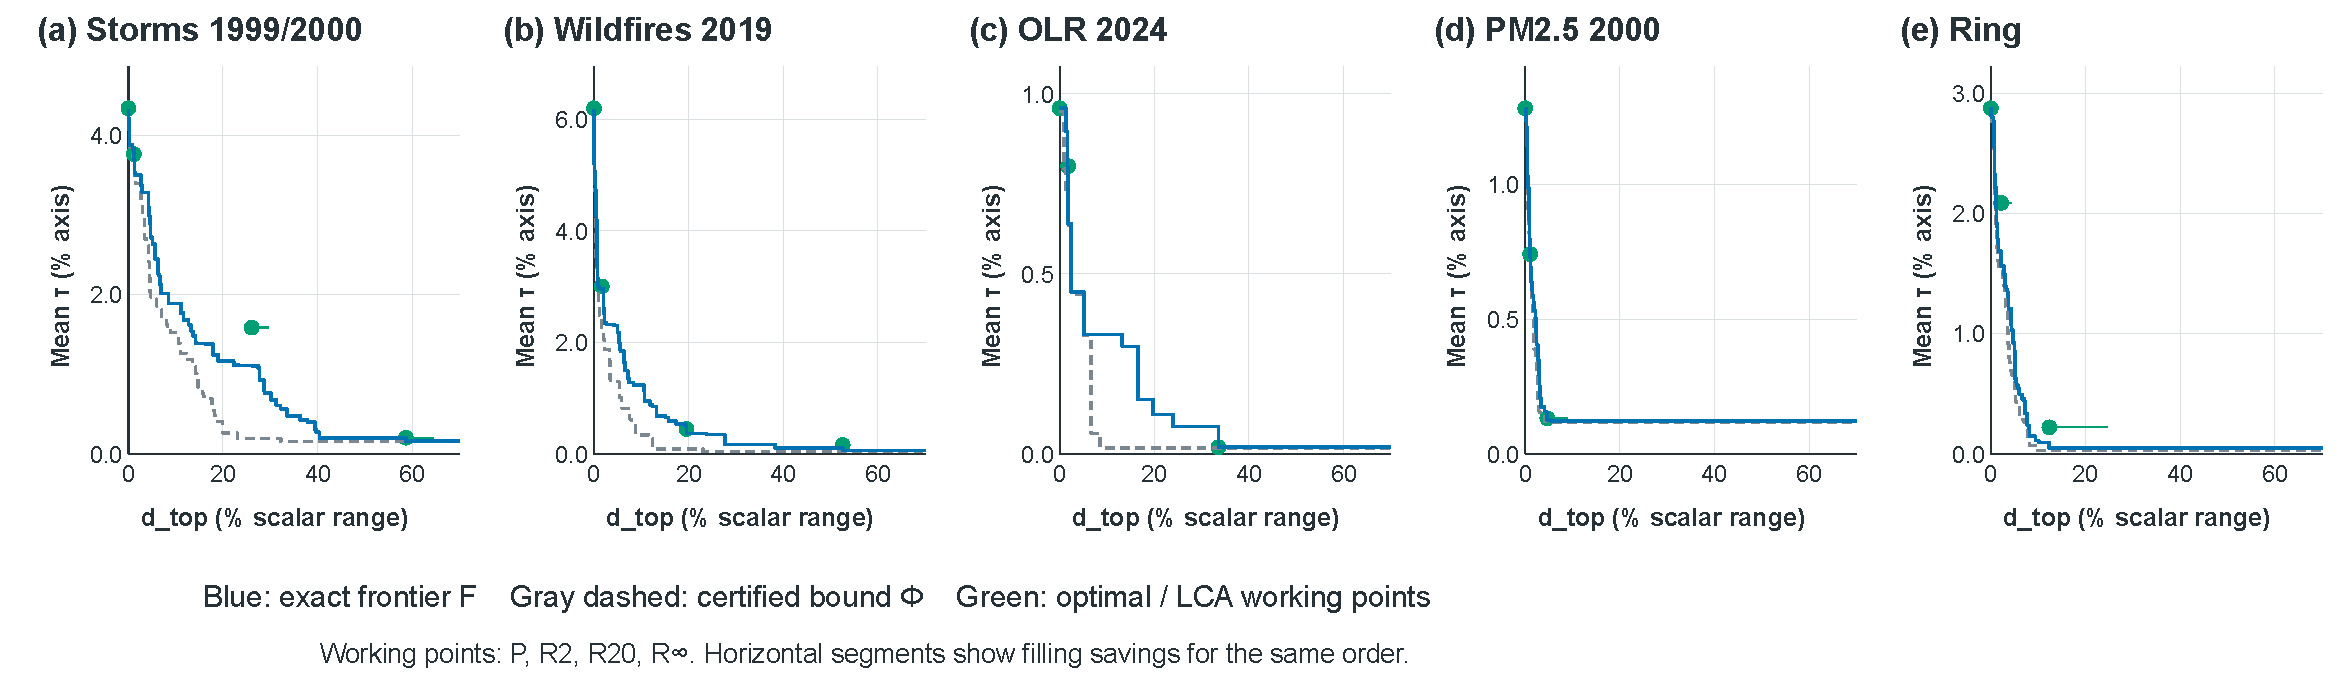
\includegraphics[width=\textwidth]{figures/Fig5.pdf}
\caption{Position--topology trade-offs for all five current planar temporal inputs, including complete-year PM2.5. Curves show temporal means of exact per-frame frontiers $F$ (blue) and certified lower bounds $\Phi$ (dashed) at a common scalar budget. Green points compare optimal (filled) and original-LCA (open) filling for identical selected orders at $\kappa/\Delta_F\in\{0,0.02,0.20,\infty\}$. Their horizontal coordinates are cross-frame maximum scalar costs; vertical coordinates are mean fixed-order position optima $\tau(\pi)$. Horizontal segments show scalar-filling savings for a fixed order. These common-budget curves differ from the per-frame 611/614 frontier-attainment check.}
\label{fig:diagnosis}
\end{figure*}

Hierarchy cost exceeds 2\% of reference extent in 40/118 Storms, 19/30 Wildfires, 7/60 OLR, 36/366 PM2.5, and 21/40 Ring frames. Hierarchy contributes more than packing in every sequence: respective mean costs are 4.17\%/0.16\% on Storms and 6.12\%/0.06\% on Wildfires; Supplement S3 retains all five pairs.

Independent LP and order-enumeration checks connect the position formulas to feasible layouts. Measured barriers agree with the optimal filling to within $1.2\times10^{-5}$ of the processed scalar range, including the strict-extremum clearance. TMTM, ST-MTM, and RG-MTM-P have zero measured labelled pairwise merge error across all suite frames. For the selected RG-MTM-R orders, fixed-order position optima reach the exact frontier within half a 1024-grid pixel in 611/614 frames. Figure~\ref{fig:diagnosis} shows all five current planar temporal sequences, including full-year PM2.5. The 611/614-frame check uses each frame's own measured scalar cost; the plotted mean curves instead use one common budget. Frontiers use one common budget; working points combine mean positional optima with maximum scalar costs. Table~\ref{tab:tradeoff} separately measures final anchors.

Holding the selected order fixed isolates scalar correction. Optimal barriers reduce mean Storms NMLE from 2.07\% for original-LCA filling to 1.47\%, and Ring from 5.46\% to 2.73\%. Packed reference sorting reaches zero Storms NROE with 6.18\% mean NMLE, compared with RG-MTM-R's 1.47\%. These controls separate the effects of reference ordering, hierarchy choice, and barrier construction.

\subsection{Retained Temporal Profiles: Reference, Geometry and Motion}
Within the five-sequence planar suite, RG-MTM-P lowers NROE relative to both baselines on every sequence while retaining the source merge levels (Table~\ref{tab:tradeoff}). Storms changes from ST-MTM's 16.28\% to 3.77\%, and Wildfires from 24.02\% to 5.83\%. This isolates the benefit of a reference-guided layout within the original hierarchy.

Relaxation improves NROE and pooled displacement on all five planar temporal sequences. Storms changes from 3.77\% to 1.16\% NROE, 4.13\% to 2.14\% pooled displacement, and 26.19\% to 18.46\% maximum displacement. Wildfires reaches 0.34\% NROE and 0.80\% pooled displacement. Table~\ref{tab:tradeoff} retain every sequence's order and coordinate measurements.

For the five planar temporal sequences, mean relaxed NMLE ranges from 0.18\% to 3.96\%, with maxima of 4.67\%--33.56\%. Storms incurs 1.47\% mean and 26.07\% maximum NMLE; Wildfires incurs 3.96\% and 19.56\%. These measured barriers quantify both sequence-wide and worst-frame costs against the source trees.

% Figure 1 shows RG-MTM-R20; the Storms four-method detail is in Supplement S8.

On Storms, motion-proxy errors decrease from ST-MTM's 43/104 to RG-MTM-R's 19/104 events. The paired difference is $-23.1$ percentage points, with a 95\% temporal-block interval of $[-33.6,-12.8]$. Ring decreases from 43/124 to 16/124. The complete table preserves each input's shared event counts and both RG modes. Tangaroa and Cylinder use three-dimensional spatial truth, whereas planar sequences use two-dimensional truth; static inputs have no temporal-motion score. Supplemental projected-motion scores use separate event populations.

On annual PM2.5, improved reference order does not yield improved spatial-motion classification: P makes 42/95 errors and R20 makes 47/95, compared with ST-MTM's 49/95. This full-year result supersedes the selected January example. Geometry remains a complementary criterion. On Wildfires, R reduces ST-MTM's SNS from 0.0786 to 0.0579 and TD from 7.9585 to 3.2487. Supplement S3 gives all geometric results, direction/persistence/extraction/eligibility controls, baseline settings, motion windows, and the separate large binary-tree benchmark.

\subsection{Absolute Reference and Hierarchical Ordering}\label{sec:reference_control}
\begin{figure*}[t]
\centering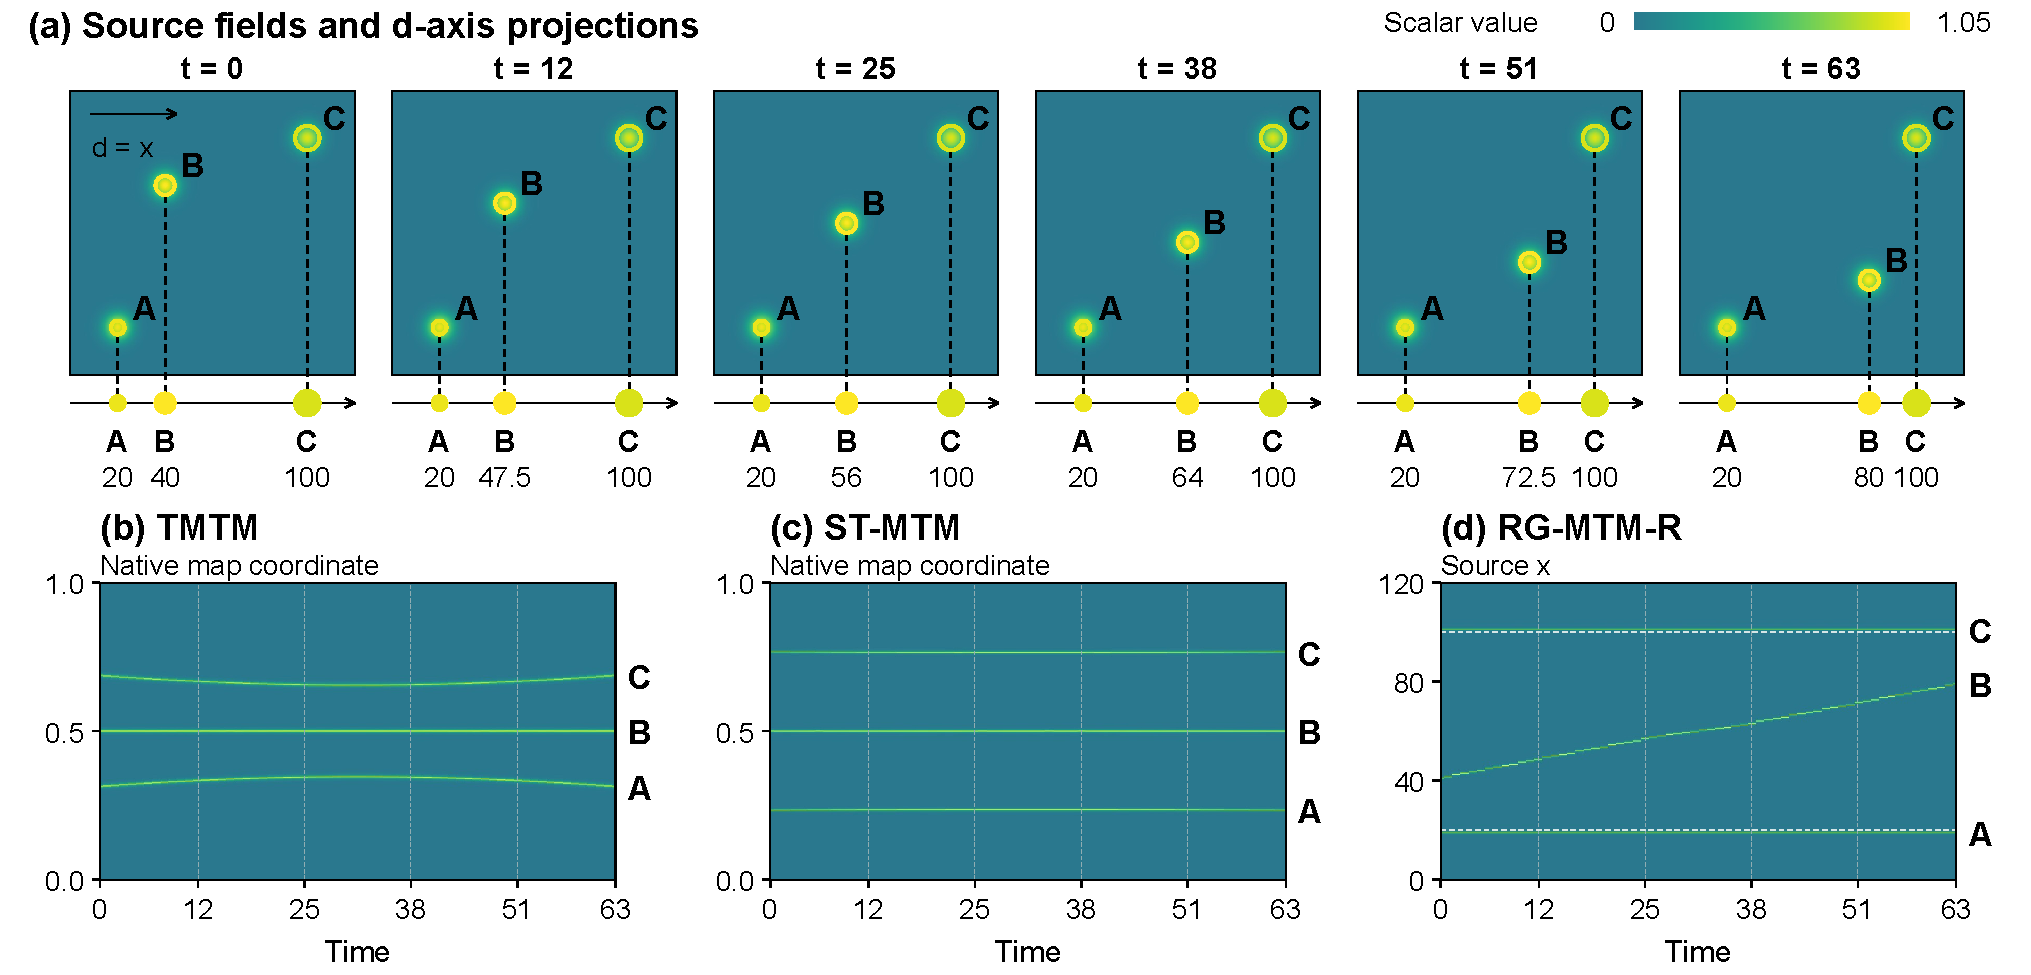
\includegraphics[width=\textwidth]{figures/Fig6.pdf}
\caption{Relative distances and absolute reference position. (a) Six source fields and $x$ projections follow moving $B$ between fixed $A,C$; mirror endpoints preserve pairwise distances while changing horizontal position. (b,c) TMTM/ST-MTM use internal map coordinates. (d) RG-MTM-R uses source $x$ units, with dashed fixed references. Source peaks and temporal bands share a linear 0--1.05 scalar scale. Vertical guides mark source-frame times. All three preserve merge levels; position errors and calibration are reported in Section~\ref{sec:reference_control}.}
\label{fig:bisector}
\end{figure*}

The mirror-motion control separates fixed-reference anchoring from pairwise-distance preservation (Fig.~\ref{fig:bisector}; protocol and measurements in Supplement S2, full visual comparison in S10). Across 64 fields on a $241^2$ grid, $B$ moves from $(40,80)$ to $(80,40)$ along the perpendicular bisector of fixed peaks $A=(20,20)$ and $C=(100,100)$. The mirror endpoints have identical distance matrices but different $q_i=x_i$. TMTM and ST-MTM keep $B$ near a constant map ordinate; RG-MTM-R follows its increasing reference. Final-frame position errors are 16.67\%, 16.67\%, and 0.84\%, using each baseline's best sequence-wide affine minimax calibration, including one global reflection. All three preserve merge levels. These 64 frames are independent of the 614-frame main suite.

\paragraph{Hierarchical row ordering.}
The certificate also diagnoses a clustering hierarchy of 1024 active wildfire cells, each containing 30 two-day observations. Optimal leaf ordering displaces some cells by 88.23\% of display height, compared with the hierarchy-constrained optimum of 67.29\% and the free-packing optimum of 20.55\%. Their separation distinguishes the chosen ordering from the cost imposed by subtree contiguity. Supplement S10 retains the full side-by-side display and protocol; S3 gives numerical precision and records.

\subsection{Data Size and Topological Complexity}
Spatial resolution determines the cost of tree extraction and the number of samples available for scalar filling; the number and branching degree of retained features determine the difficulty of positional diagnosis and order selection. Raster resolution controls how finely anchors and barriers appear in the final map. These are separate scales: a large input volume need not require exhaustive ordering of all its samples.

The retained binary-hierarchy benchmark increases from 64 leaves on 256 rows in 0.0041\,s to 4096 leaves on 16384 rows in 3.604\,s. These measurements concern positional diagnosis in the recorded benchmark environment. They do not include field preprocessing, scalar filling, or the quadratic layout. Exact small-tree frontiers enumerate permutations; flattening nodes can increase branching degree and the cost of subset-based diagnosis. The degree-controlled benchmark and timing details are in Supplement S3.

